\documentclass[twoside,a4,12p]{report} %,draft,openright]

\usepackage{epsf,graphicx}
\usepackage{latexsym,amssymb}
\usepackage{setspace,cite}
% for margins left, right top bottom
\usepackage{anysize}
\marginsize{4cm}{2.5cm}{4cm}{4cm}

%\usepackage{draft} %draft option - doesn't put full figures in -
            % useful when editing

%does the headers on the pages - keep in
\usepackage{fancyhdr}

\begin{document}
\newpage

%Puts page numbering of preamble in roman and of main body of thesis in
%arabic. Also defines how chapters and sections are made
\pagenumbering{arabic}
\setcounter{page}{1} \pagestyle{fancy}
\renewcommand{\chaptermark}[1]{\markboth{\chaptername%
\ \thechapter:\,\ #1}{}}
\renewcommand{\sectionmark}[1]{\markright{\thesection\,\ #1}}

% ===================================================
%%%%%%%%%%%%%%%%%%%%%%%%%%%%%%%%%%%%%%%%%%%%%%%%%%%%%%%%%%%%%%%%%%%%%%%%%%%
% Juan Manuel Perez Rua
%%%%%%%%%%%%%%%%%%%%%%%%%%%%%%%%%%%%%%%%%%%%%%%%%%%%%%%%%%%%%%%%%%%%%%%%%%%

\newpage
\thispagestyle{empty}

% ******* Title page *******
% **************************

\vspace*{1cm}
\begin{center}
{\huge\bf OBJECT FLOW\\}
{\large\bf A per-object dense motion descriptor\\}
\vspace{2cm} 
{\large Juan Manuel P\'erez R\'ua\\}
\vspace{1cm} 

\includegraphics[height=0.15\textheight]{images/logo/technicolor_large.png} \\
\includegraphics[height=0.1\textheight]{images/logo/ubourgogne.png}

\vspace{2cm} 
\normalsize{Technicolor SA  - University of Burgundy \\}
\end{center}

\vspace{2cm}
\begin{center}
{\large A Thesis Submitted for the Degree of \\MSc Erasmus Mundus
in Vision and Robotics (VIBOT) \\\vspace{0.3cm} $\cdot$ 2014
$\cdot$}
\end{center}
\singlespacing

\begin{abstract}

Motion analysis in image sequences has undoubtedly shown good 
progress in terms of its two main research branches. 
Optical flow estimation and object visual tracking have been 
mostly studied as isolated problems, and high accuracy algorithms 
are available when needed as independent bricks. 
This paper presents a framework for combining object tracking 
techniques with optical flow methods aiming towards a precise 
motion description for objects in video sequences. 
Firstly, we introduce a method to extend max-flow min-cut based 
segmentation techniques to videos, without adding the computational 
load of performing a graph cut optimization approach for 3-dimensional
graphs. 
This is done by exploiting the inherent foreground-background 
separation hints given by object trackers, and the novel concept 
of super pixel flow. 
Then, we show that long-motion awareness obtained from object 
tracking, together with a per frame object segmentation can 
improve the precision of the object motion description in 
comparison to several optical flow techniques. 
We may call the proposed approach “Object flow” as it offers a 
dense and semantic aware description of the current motion state 
of the studied object. 


\end{abstract}
% ===================================================
\doublespacing

%\pagestyle{empty}
\pagenumbering{roman}
\setcounter{page}{1} \pagestyle{plain}


\tableofcontents
\listoffigures
%\listoftables

%\chapter*{Acknowledgments}
%\addcontentsline{toc}{chapter}
%         {\protect\numberline{Acknowledgments\hspace{-96pt}}}
%

\pagestyle{fancy}
% ===================================================

\newpage

\addtolength{\headheight}{3pt} \fancyhead{}
\fancyhead[LE]{\sl\leftmark} \fancyhead[LO,RE]{\rm\thepage}
\fancyhead[RO]{\sl\rightmark} \fancyfoot[C,L,E]{}
\pagenumbering{arabic}

% ===================================================
%\singlespacing
%\doublespacing
\onehalfspacing
\section{INTRODUCTION}
\label{sec:introduction}
Superpixels and over segmentation techniques
became a widely used pre-processing stage for a
large number of machine vision applications, after the
original concept was introduced \cite{c1}. Superpixels are
traditionally used as performance booster for several
other techniques. However, it is still mostly related to
single frame processing \cite{c1}\cite{c10}\cite{c11}. In the search for
consistency in superpixel labeling through video,
some authors have proposed different techniques,
which go from simple extension to supervoxels\cite{c9}\cite{c11},
to more complicated approaches \cite{c8}. These
approaches, nonetheless, usually require a global
processing and knowledge of all (or several of) the
video frames beforehand. One of the contributions of this work is a superpixel
matching technique which assumes a flowlike
behavior in the image sequences (natural video), and
propose an application for improving object segmentation in videos.

For some kind of video sequences and computer vision
applications the superpixel labelling usually loses coherency between frames, 
even when computed as supervoxels. 
This means superpixel matching techniques offer some interest and can still be
explored. Some work have been done towards a
superpixel based image comparison using the Earth
Mover's Distance, by taking super pixels as bins of a
global histogram \cite{c2}. The label propagation or superpixel flow can be
achieved with this technique by selecting the superpixel in the second frame that maximize the flow
from each superpixel in the first frame.
However, we look at the problem of superpixel
propagation between a pair of frames, in terms of the
indexes of the already computed superpixelization in
both of them. \\
By taking into account superpixels computed separately in images we can open the advantages of
streaming like approaches, so the video process can be performed by processing only two frames at a time, 
saving memory and moving towards a more time friendly approach. This propagation means finding
the superpixel labels in the second frame that
correspond to a given label in the first frame. This
matching, however, has to comply with a set of
constraints. Firstly, two correspondent superpixels
should be similar in terms of some appearance
feature, which most likely depends on the way the
superpixelization was performed (color, texture,
shape). Also, the superpixel propagation should
maintain certain global homogeneity (at least for
superpixels that belong to the same object). This is
because the superpixel propagation or matching is
not completely a one-to-one combinatorial problem,
but more a “superpixel flow”. In this sense, it seems
natural that the problem of superpixel propagation
could be solved with a discrete energy minimization
procedure. If the size compactness of the superpixels is maintained, 
it actually seems to share some of the properties of the
optical flow problem, with the difference that the
smoothness is usually a very strong constraint for the
last one. The strength of this smoothness prior relies
not only in the nature of the problem, but also
because it gives better cues towards an easy-to-
minimize global approach.
\chapter{Background and Related Work} \label{chap:background}

\section{Introduction}

The background of the object flow concept is mainly related to object tracker techniques and optical flow methods. A short state of the art review is presented in 
following sections, without going too deeply in any specific approach, since those are widely diverse. Of course, another important point is the object based segmentation in videos problem. Several works have involved this or similar problem in 
the state of the art, and only the more related approaches are presented. On the other hand, as the object flow itself is a novel method, the related work is not large.
 However, as, in terms of applications, some works have been done towards specific oncomings to this concept. Some of these are superficially explained.

\section{Object Tracking}

   \begin{figure}[thpb]
      \centering
      \includegraphics[width=1.0\textwidth]{../images/tr_db.png}
      \caption{Sequences used to evaluate object trackers in \cite{c16}. }
      \label{tr_db}
   \end{figure}

As one of the most studied computer vision problems, object tracking has been constantly evolving since its early approaches. 
As the techniques were getting better, the benchmarking has been evolving too. The last global work in online object tracking 
was the work of Wu et al. \cite{c16} in 2013. Several remarks can be extracted from the deep benchmarking analysis of this work. 
For instance, it seems to be more clear that background information is a key hint towards 
better tracking methods. Some kind of modelling of the background should be an important 
step in the tracking pipeline. Whether this background modelling is implicit like in \cite{c23} or 
explicit like in \cite{c22}, where is used as context, is just matter of design. Of course, this 
background modelling have to be accompanied with local model to account with variations (occlusions, deformations) in the interest object. 
It seems that these two are the reasons why tracking by detection and learning approaches are among the most successful ones. Usually, 
these methods account with local and background modelling (\cite{c22}\cite{c23}\cite{c24}\cite{c25}\cite{c26}). 
However, even when motion or dynamical models is crucial for object tracking, very few of the last state of the art techniques focus on this 
element. The Fig. \ref{tr_per} shows results for the top 15 state of the art trackers as presented in \cite{c16}, taking into account 
the variability of different initialization. According to this data, the tracking problem is still open and further exploration can be done. 
Moreover, it has to be observed that tracking by detection methods are indeed in the top of results in stability in initialization and peak performance. 
The Struck tracker \cite{c23}, for instance, seems to hold the higher position w.r.t stability. Another curious observation is the fact that even traditionally good color based particle filter approaches are left behind with last years object trackers.

   \begin{figure}[thpb]
      \centering
      \includegraphics[width=1.0\textwidth]{../images/trackers_performance.png}
      \caption{ Performance summary for the top 15 trackers benchmarked in \cite{c16}, initialized with different size of bounding box. }
      \label{tr_per}
   \end{figure}

\subsection{Tracking-by-detection methods}

Current tracking methods look at the problem as a classification task and use online learning techniques to update the object model \cite{c23}. The main reasons for the success of these approaches are the recent advances in object detection
methods ({\it boosting}, {\it SVM}) and fast learning algorithms. 
The normal 
flow on these methods includes to 
sample the image to create a list 
of labelled training examples. 

   \begin{figure}[thpb]
      \centering
      \includegraphics[width=0.66\textwidth]{../images/tbd.png}
      \caption{Usual approaches for tracking-by-detection methods. Right: generate a set of samples and, depending on the type of learner, produce training labels. Left: Structured output methods avoid these steps by operating directly in the tracking output. Extracted from \cite{c23}.}
      \label{tr_tbd}
   \end{figure}


Usually, the position of the object 
is computed from the sample with the maximum classification score in a local window. 
This method, however, is not perfect, and most of the methods 
focus on increasing the robustness 
of the classifier to poor labelling 
and sampling, by including semi-supervised learning, robust statistics or multiple-instance 
learning \cite{c25}. Other approaches deal with these problems 
in a whole different way. For instance, the use of structured learning seems to outperform most 
of the tracking-by-detection methods \cite{c23}. In this way, 
the tracking is defined directly 
as predicting the change in object location between frames, by the use 
of structured output spaces (the same that is used in applications like text translation). Fig. \ref{tr_tbd} shows a diagram of most used approaches to tracking-by-detection methods. 
   
\section{Optical Flow}

   \begin{figure}[thpb]
      \centering
      \includegraphics[width=1.0\textwidth]{../images/of_db.png}
      \caption{Frame pairs used to evaluate optical flow methods in \cite{c17}, Ground truth flow coded with the proposed flow coding. }
      \label{tr_db}
   \end{figure}

Optical flow is another traditional problem in computer vision, and it may be argued that its under-determined nature makes it one of the most difficult ones. 
Several well known databases and benchmarks have been proposed to account for the different intrinsic complications of the problem. The last and larger benchmarking 
work for this problem may be Baker et al. \cite{c17}, but other useful studies are available \cite{c27}. 
These works reveal that most of the existing methods establish the problem as the optimization of an energy function that takes into account two terms. The first one, $E_{data}$ 
measures data consistency over input frames, and $E_{prior}$ which favours flow with certain characteristics, e.g. smoothness in the flow. It seems that one of the major 
challenges remains to be the best pair of objective function and optimization method. A number of combinations have been proposed \cite{c29}\cite{c30}\cite{c32}. However, 
totally different approaches had been also proposed, e.g. by using polynomial expansions \cite{c28}.

\begin{equation}
E_{global} = E_{data} + \lambda E_{prior}
\label{eq_ener}
\end{equation}

According to the update of 2011 of the work in \cite{c17}, the first 15 optical flow methods by interpolation error are shown in the Fig. \ref{of_per}. It has to be noted that the performance in several of the dataset is already very good for the most of these methods.

   \begin{figure}[thpb]
      \centering
      \includegraphics[width=0.8\textwidth]{../images/of_performance.png}
      \caption{ Performance summary for the top 15 opt. flow methods benchmarked in \cite{c17} by interpolation error. }
      \label{of_per}
   \end{figure}

\subsection{Simple Flow}

As the Simple Flow \cite{c21} is the optical flow technique that is used as base of the proposed 
object flow method, it is presented in more detail. 
The main characteristic of this method is its efficient approach, which tries to concentrate in the zones where there is evidence of motion, and use linear 
interpolation for excluded zones. 
Moreover, the problem is not solved in the usual way by minimizing a variation of (\ref{eq_ener}), but using a simpler likelihood model that 
follows the constant-color assumption, without including explicitly the pairwise terms that account for smoothing. The smoothness prior it is taken into 
account, however, by implementation of local filters that uses pixel weighting to take into account pixel proximity ($w_d$) and color similarity ($w_c$)., leading to a equation 
of the type: 

\begin{equation}
E(x_0, y_0, u, v) = \sum_{(x,y) \in \mathcal{N}_{0}} w_{d}w_{c}||  I_{0}(x,y) - I_{1}(x+u,y+v) ||^2
\label{eq_simple}
\end{equation}

   \begin{figure}[tbhp]
      \centering
      \includegraphics[width=0.85\textwidth]{../images/simpleflow.png}
      \caption{  Results of the Simple Flow method in several datasets. }
      \label{simple_of}
   \end{figure}

   \begin{figure}[tbhp]
      \centering
      \includegraphics[width=0.95\textwidth]{../images/simpleoptflow.png}
      \caption{  Results of the Simple Flow method in several datasets. }
      \label{simple_of}
   \end{figure}

The practical implementation of this equation requires a cross-bilateral filter to compute $E$, as it takes into account 
pixel $(x_0,y_0)$ centred $nxn$ windows between $I_0$ and $I_1$, producing $n^2$-dimensional vector for each pixel. 
The flow is the vector $(u_0, v_0)$ that minimized $E$, producing an integer value. The precision can be enhanced by fitting 
parabolas at  $(u_0, v_0)$ and extracting the minimum. A final bilateral filtering is applied to the flow field, discarding 
occluded pixels (determined by cross-matching using the computed forward and backward flows). 
To recover large motions, instead of using large $nxn$ windows, a multi scale approach is followed. 
If more accuracy is desired, a more global optimization can follow, for instance, connecting the global approach used in Sun et al. \cite{c40}.
This simple approach for computing optical flow ranked in a very good position in the Middlebury evaluation \cite{c17}, 
and some results can be appreciated in the Fig. \ref{simple_of}.

\section{Object segmentation in video}

Among the state of the art segmentation methods for objects in video
sequences, point trajectories based ones stand for its performance and 
reliability \cite{c33}, even when only sparse trajectories are known because of
computational reasons \cite{c34}. On the other hand, for the problem of extracting out a 
preselected object in still frames, max-flow min-cut based approaches 
have demonstrated to be a powerful tool \cite{c14}\cite{c18}. 

   \begin{figure}[thpb]
      \centering
      \includegraphics[height=0.28\textheight]{../images/point_traj_segm.png}
      \caption{  Sparse motion trajectories for segmentation. Results in several datasets  \cite{c34}. }
      \label{pt_seg}
   \end{figure}


The Fig. \ref{pt_seg} shows good accuracy results when using sparse motion trajectories \cite{c34}. However, to overcome 
the sparsity of the flow the authors proposed a variational method to obtain density. The information propagation is done 
by presenting the problem as a non-linear diffusion process that takes superpixels into account. It is expected, then, that this 
method can be precise, but slow.
In this work we propose to mix single frame graph based approaches with the idea 
of using background point trajectories. However, the sparsity of point trajectories is 
overcame by using superpixels. Therefore, instead of tracking points, background regions are tracked via the novel concept of 
superpixel flow. 
We show in future sections how this extra information can be used to complement the
graph-cuts based techniques for an efficient foreground-background segmentation. 

\section{Related work}

As previously mentioned, the related work is commented mostly from an application-wise point-of-view, due to the fact that 
the object flow concept is novel. The most used approaches in the literature to mix motion estimation with scene semantics 
are related to the use of this motion estimation to perform segmentation of scene \cite{c33}\cite{c34}. These works, however, depend 
intrinsically in the accuracy of the motion estimation to perform a good segmentation. Other authors have proposed to use simple 
low-order parametric motion models to model background movement, and by incorporating radial maps, obtain a frame-by-frame 
moving object segmentation \cite{c36}, in contrast with the methods that combine motion awareness with appearance information \cite{c35}. 

From other point of view, regarding the problem of large displacement motion estimation, the use of superpixels seems to provide a reliable hint. The work presented in \cite{c39} 
provide an interesting method to combine the idea of optical flow with superpixels, to obtain an optical flow method which can perform well in difficult datasets \cite{c27}. 
The full set of these ideas can lead to some conclusions towards the object flow pipeline proposal. For instance, authors have already exploited the optical flow 
to improve tracking methods. It remains unexplored to complete the cycle by improving the optical flow with the state of the tracker. Moreover, these works have shown 
that the use of superpixels can be combined with motion estimation to obtain both an object based segmentation and the enhancement of the motion itself.

On the other hand, other authors had used the optical flow constraints to track objects, 
which is, up to some extent, the inverse problem proposed for the object flow \cite{c37}. Some authors went further in this sense, to create specialized trackers 
for deformable objects by combining model based tracking with the optical flow constraint \cite{c38}. Even when a work like the last one is very interesting for video editing 
tasks, the approach is limited by the availability of the mesh model. In this sense, the object flow proposal seems to be more generic, and thus, more adequate for this kind 
of applications. The Fig. \ref{soa1} shows some results of this approach for the video edition tasks that can also be approached with the object flow. These results are obtained in 
a controlled environment without long range motion.

   \begin{figure}[thpb]
      \centering
      \includegraphics[width=0.75\textwidth]{../images/soa_app.png}
      \caption{  Video edition with the method in  \cite{c38}. }
      \label{soa1}
   \end{figure}

In the same line of applications, an interesting work is the Unwrap Mosaics \cite{c41} which is a very different way to approach the video edition task. 

   \begin{figure}[thpb]
      \centering
      \includegraphics[width=1.00\textwidth]{../images/soa_app2.png}
      \caption{  Video edition with the method in  \cite{c41}. }
      \label{soa2}
   \end{figure}

The Unwrap Mosaics \cite{c41}, is based in a new 
video representation, which is presented by defining a 2D-2D transformation supported in a segmentation mask (given by hand), which can be used to apply the desired editing in the 
interest object, and then, given the compute transformation, the edition can be mapped back to the initial sequence. The Fig. \ref{soa2} shows the video edition flow derived from 
this method. However, relying in precomputed segmentation and point trajectories, the Unwrap Mosaics can be mixed with the Object Flow pipeline to provide a robust and 
complete video edition framework.
%%%%%%%%%%%%%%%%%%%%%%%%%%%%%%%%%%%%%%%%%%%%%%%%%%%%%%%%%%%%%%%%%%%%%%%%%%%
% Juan Manuel Perez Rua
%%%%%%%%%%%%%%%%%%%%%%%%%%%%%%%%%%%%%%%%%%%%%%%%%%%%%%%%%%%%%%%%%%%%%%%%%%%

\chapter{Object Flow Pipeline} \label{chap:core}
Following the definition of the problem given in the Section \ref{sec:definition}, a 
 system for computing the object flow have been devised. 
 This system is composed of three  main steps, which will be explained in short.  
 
\section{Algorithm description}
\label{sec:desc}

Fig. \ref{figurelabel_sys} shows a simplified block diagram of the proposed system. It is important to recognize the two main 
components of our work-flow: object tracking and segmentation, and pixel-wise flow computation on the pixels of interest.  The scheme is completed by feeding back the flow 
information to improve the tracker as depicted in the figure. For instance, one can make the most of dense displacement vectors to refine the motion of the target, and 
the segmentation information can be used to improve the sampling process of the learning stage in several trackers by detection methods \cite{c22}. Thus, 
the tracker and motion flow algorithm can work for mutual enhancement.

   \begin{figure}[thpb]
      \centering
      \includegraphics[width=1.00\textwidth]{../images/system.png}
      \caption{Block diagram of the proposed pipeline.}
      \label{figurelabel_sys}
   \end{figure}

 The object tracking in the object flow pipeline can be selected according to a specific need for a given application. Here, recent methods based on tracking-by-detection are preferred, given that they are in the top of modern benchmarks for object tracking \cite{c16} in terms of accuracy and stability to initialization changes. Even more, as previously mentioned 
tracking-by-detection techniques benefit from the background-foreground separation of the next stage in the object flow pipeline. For instance, the sampling process in the {\it Struck} 
tracker can be improved by selecting positive samples only inside the region of the target object.
In the second place, for the object segmentation in video, the 
labelled background regions through the concept of superpixel flow, as explained in 
Section \ref{chap:suppix}, is shown. The last step, the flow computation, uses a modified 
{\it Simple Flow} algorithm, which uses the provided segmentation masks for an accurate estimation.

%\section{Superpixel propagation for object segmentation in videos}
% \subsection{Background regions tracking for object segmentation}
\label{sec:segm}
Determining the spatial support of the object in a given frame benefits from the output of the tracker. Appearance cues alone, learned inside and outside the tracking window can result in a misleading modeling of the foreground and the background. In contrast, we propose to perform foreground-background segmentation by tracking background pixels surrounding the target, thanks to the tracker output. Thus, the pixels that are initially outside the tracker window, 
are followed through the sequence and as long as they enter the tracked region, they can be safely labeled as background. This idea can be observed in the Fig.  \ref{figurelabel_entering}, 
where the object window given by the tracker (green) loosely separates the foreground from the background. Points outside the tracker (blue) are labeled as background in previous frames, and as they enter the tracker window (red points), they can be used to improve the modeling  of the foreground and the background. The red window is used to save computational power by avoiding to track points that are too far from the interest object.

\ifcsdef{r@accv_format}{
   \begin{figure}[thpb]
      \centering
      \includegraphics[height=0.175\textheight]{../images/tracking_points.png}
      \caption{Example image of points entering a tracking region (green) due to object motion in a video sequence.}
      \label{figurelabel_entering}
   \end{figure}
\setlength{\belowcaptionskip}{-10pt}
}{
   \begin{figure}[thpb]
      \centering
      \includegraphics[width=0.5\textwidth]{../images/tracking_points.png}
      \caption{Example image of points entering a tracking region (green) due to object motion in a video sequence.}
      \label{figurelabel_entering}
   \end{figure}
\setlength{\belowcaptionskip}{-10pt}
}

Tracking pixels as independent points, however, carries several problems. First, to track all the background points means to compute the optical flow between the image pair, which can become very inneficient 
when taking into account large objects. Second, the point tracking techniques causes some drift in the trajectories, which can lead to wrong labelling as background. Finally, the background labelling could be 
more dense, and less complex if superpixels are tracked instead of pixels.  After several frames, 
the labeled superpixels will almost completely cover the unwanted areas in a dinamyc scene. We call this process background segments tracking.  Fig. \ref{figurelabel_spflow} shows this idea in a real scenario. From left to right, initially the superpixels with elements outside the bounding box are labeled as background (green), then, as the sequence runs, the labeled superpixels flow inside the window, propagating the background mask. 
The segmentation is then refined  applying the grab-cut method (\cite{c18}\cite{c15}) guided by the background labeling, which works a an initialization, replacing the usual user interaction.

\ifcsdef{r@accv_format}{
   \begin{figure}[thpb]
      \centering
      \includegraphics[width=0.95\textwidth]{../images/suppixflow2.png}
      \caption{Background segments automatic labeling and propagation, the flow goes from left to right. The superpixels that are outside the tracker window (yellow) are labelled as background (green) in the first frame. These labels are propagated 
when the sequence runs.}
      \label{figurelabel_spflow}
   \end{figure}
}{
   \begin{figure}[thpb]
      \centering
      \includegraphics[width=0.5\textwidth]{../images/suppixflow2.png}
      \caption{Background segments automatic labeling and propagation, the flow goes from left to right. The superpixels that are outside the tracker window (yellow) are labelled as background (green) in the first frame. These labels are propagated 
when the sequence runs.}
      \label{figurelabel_spflow}
   \end{figure}
}

%\subsection{Superpixel flow}
\label{sec:suppix}
%As a preprocessing step in the object flow pipeline, we propose a superpixel matching technique which assumes a flowlike behavior in the image 
%sequences (natural video), which can be used to track superpixels. 
%This matching, however, has to comply with a set of constraints. 
%Firstly, two correspondent superpixels should be similar in terms of some appearance
%feature, which most likely depends on the way the superpixelization was performed (color, texture,
%shape). Also, the superpixel flow  should maintain certain global regularity (at least for
%superpixels that belong to the same object). %In this sense, it seems

%If the size compactness of the superpixels is maintained,  it actually seems to 
%share some of the properties of the optical flow problem, with the difference that the
%smoothness is usually a very strong constraint for the last one. 
%The strength of this smoothness prior relies not only in the nature of the problem, but also
%because it gives better cues towards an easier-to-minimize global approach.

In order to perform the background segments tracking,  we propose a superpixel matching technique, 
which we call superpixel flow. The objective of the superpixel flow is to find the best match for every superpixel $p$ in the first 
frame with one ($p'$) in the next frame, while holding a global flow-like behaviour.

Thus, the superpixelization should maintain certain size homogeneity within a single frame. Some super
pixel techniques can cope with this requirement \cite{c9}\cite{c10}. For the experiments presented 
in this work, we prefer the SLIC method \cite{c9}, which gives
good results in terms of size homogeneity and compactness of the superpixelization. 

%\subsection{Energy Formulation}

Inspired by a large number of optical flow and stereo techniques \cite{c7}\cite{c12}\cite{c13}, 
the superpixel flow is modelled with a pairwise Markov Random Field. The matching is performed via maximum-a-posteriori (MAP) inference on the labeling $l$, which is equivalent to the minimization of an energy function of the form:

\begin{equation}
E(l) = \displaystyle \sum_{p \in \Gamma} D_p(l_p;I_0,I_1) +
\sum_{(p,q): q \in \mathcal{N}_r} S_{p,q}(l_p,l_q) .
\label{eq_energy}
\end{equation}

With $l$ the set of labels of the superpixels in $I_0$,
that match with those in $I_1$. $\mathcal{N}_r$ is a neighbourhood of radius $r$ of the superpixel $p$.
The terms $D$, and $S$ in (\ref{eq_energy}) stand for data term and spatial smoothness term. 
The first one determines how accurate is the labeling in terms
of consistency with the measured data (color, shape,etc.). In the classical optical flow equivalent of this equation,
the data term corresponds to the pixel brightness conservation\cite{c7}\cite{c5}. However, as superpixels are a set
of similar (or somehow homogeneous) pixels, an adequate appearance based feature is a low dimensional
color histogram (with N bins). So, here, $D$ is the Hellinger distance between the histograms:

\begin{equation}
D_p(l_p;I_0,I_1) = \sqrt{ 1 - \frac{1}{\sqrt{\bar{ \boldsymbol{h} }(p) \bar{ \boldsymbol{h} }(p')N^2} } \sum_{i}\sqrt{ \boldsymbol{h}_{i}(p) \boldsymbol{h}_{i}(p')} }.
\label{eq_Dp}
\end{equation}
Where $\textbf{h}(p)$ and $\textbf{h}(p')$ are the color histograms of the superpixel $p$ and its correspondent superpixel in the
second frame $I_1$. For the experiments we used {\it RGB} color histogram with N=3 bins per color.
Note that the low dimensional histogram gives certain robustness against noise,
and slowly changing colors between frames. 

On the other hand, the spatial term is a penalty function for spatial diference of the displacement vectors between neighboring superpixels, where a displacement vector has origin 
in the centroid of the superpixel of the first frame and
end in the centroid of the superpixel of the second frame.

\begin{equation}
S_{p,q}(l_p, l_q) = \lambda(p)
  \sqrt{\frac{|u_{p_c}-u_{q_c}|}{\|p_c-q_c\|}+ \frac{|v_{p_c}-v_{q_c}|}{\|p_c-q_c\|}},
\label{eq_Spq}
\end{equation}
 where, $ \lambda(p) = (1 + \rho(\boldsymbol{h}(p),\boldsymbol{h}(q)))^2 $.

The operator $\rho$ is the Hellinger distance as used in the
data term (\ref{eq_Dp}). The histogram distance is nonetheless computed between adjacent superpixels $p$ and $q$, 
which belong to the first image. The superpixels centroids are noted as $q_c$ and $p_c$, 
and $u_{*}$ and $v_{*}$ are the horizontal and vertical changes between centroids.
This term has a smoothing effect in superpixels that belong to the
same object. It has to be observed that when two close superpixels are different, thus, more probable to
belong to different objects within the image, the term $\lambda$ allows them to have
matches that do not hold the smoothness prior with the same strength. 

%\subsection{Energy Minimization}
\ifcsdef{r@accv_format}{
   \begin{figure}[thpb]
      \centering
      \includegraphics[width=0.935\textwidth]{../images/all_matches.png}
      \caption{The yellow lines show selected superpixel
		matching between pairs of images in several datasets.}
      \label{figurelabel_matchessnow}
   \end{figure}   
	\setlength{\belowcaptionskip}{-10pt}
}{
   \begin{figure}[thpb]
      \centering
      \includegraphics[width=0.5\textwidth]{../images/all_matches.png}
      \caption{The yellow lines show selected superpixel
		matching between pairs of images in several datasets.}
      \label{figurelabel_matchessnow}
   \end{figure}   
	\setlength{\belowcaptionskip}{-10pt}
}

The Quadratic Pseudo-Boolean Optimization (QPBO) \cite{c3}\cite{c4} is used to minimize the proposed energy function, 
by merging a set of candidate matches for every superpixel in the first frame. The candidate matches are generated by assuming 
a proximity prior. This means, every possible match should be inside a seach radius in the second frame. Fig. \ref{figurelabel_matchessnow} shows matching results for several datasets. Observe that the matches are correct even in difficult cases (bottom right).


\ifcsdef{r@accv_format}{
   \vspace*{-0.2cm}
   \begin{figure}[thpb]
      \centering
      \includegraphics[width=0.775\textwidth]{../images/Sequence2.png}
      \caption{Segmentation through the sequence “Walking
	       Couple” (Yellow contour) initialized in the man’s head. The yellow box correspond to the tracker output.
	        The labeled background superpixel are not shown for clarity.}
      \label{figurelabel_walking}
   \end{figure}
}{
   \begin{figure}[thpb]
      \centering
      \includegraphics[width=0.5\textwidth]{../images/Sequence.png}
      \caption{Segmentation through the sequence “Walking
	       Couple” (Yellow contour) initialized in the man’s head. The yellow box correspond to the tracker output.
	        The labeled background superpixel are not shown for clarity.}
      \label{figurelabel_walking}
   \end{figure}
}

Fig. \ref{figurelabel_walking} shows segmentation results for an image sequence where the interest object is the head of a person.
The head tracker and the superpixel flow provide information for better background-foreground separation. The method is tested in the Walking Couple sequence, by allowing only a small amount of iterations in the
grab-cut segmentation. Observe how the contour in the man's head is correctly delineated when
another person's head occludes part of it. In this case, the superpixels that belong to the woman’s face
were correctly propagated and thus, labeled as background, despite the similar (skin) color between foreground and background regions.

In order to understand the effect of including superpixel propagation in a video sequence for object
segmentation, some results are shown in the Fig. \ref{figurelabel_comp}. For these experiments only one iteration is
allowed in the graph-cut based methods. The top row frames (Fig. \ref{figurelabel_comp}) were initialized only with the tracker, 
and the bottom row was initialized with the superpixel tracking technique. 
Observe that in general, the contour delineated is usually better in terms of precision and
stability for the later one.
\vspace*{-0.5cm}
\ifcsdef{r@accv_format}{
   \begin{figure}[thpb]
      \centering
      \includegraphics[width=1.0\textwidth]{../images/compareSegm2.png}
      \caption{Face segmentation in the Snow Shoes sequence and T-shirt extraction from 
	      “Tennis” sequence in several frames. For each
	       group, the Top Row: One-iteration grab-cut initialized with tracker window;
	       and the Bottom Row: One-iteration grab-cut initialized with the background regions tracking.}
      \label{figurelabel_comp}
   \end{figure}
}{
   \begin{figure}[thpb]
      \centering
      \includegraphics[width=0.5\textwidth]{../images/Compare.png}
      \caption{Face segmentation in the “Amelia Retro” and the
	      “Snow shoes” sequences in three different frames. For each
	       group, the Top Row: One-iteration grab-cut initialized with tracker window;
	       and the Bottom Row: One-iteration grab-cut initialized with the background regions tracking.}
      \label{figurelabel_comp}
   \end{figure}
}

\section{Flow estimation}
%\subsection{Flow estimation}
\label{sec:core}

The object flow consist on computing the motion field for an object of interest through an image
sequence. The most usual approach to solve a problem like this is to implement some of the available
optical flow techniques through the complete sequence and perform the flow integration. 
However, this process results in high levels of motion drift \cite{c18}\cite{c19} and usually the motion of the interest
object is affected by a global regularization. In some extreme cases, the interest object motion
may be totally blurred and other techniques have to be incorporated. Moreover, the diversity
of natural video sequences makes difficult the choice of one optical flow technique over another, even when specialized
databases are at hand \cite{c17}, because currently no single method can achieve a strong 
performance in every of the available datasets. Most of these methods consist in the minimization 
of an energy function with two terms (As was previously mentioned in the Sec. \ref{sec:suppix}). The data
term is mostly shared between different approaches, but the prior or spatial term is different, and basically states 
under what conditions the optical flow smoothness should be maintained or not. In a global approach, however,
this is a difficult concept to define. Most of these smoothness terms rely in appearance differences or gradients.
All these meaning that, unavoidably, some methods may be more reliable for some cases but weaker for others. 
It can be argued that this behaviour may be caused because most of the techniques do not count with a way to identify 
firmly where exactly this smoothness prior can be applied. 

It is difficult, nevertheless, to blame the authors for the choice of some regularization 
terms, since the more robust the regularization terms is, and the higher level knowledge is applied, the more difficult is to minimize the 
energy function, and thus, the more difficult is to obtain a reliable global solution. 
The modern advances in non-convex optimization methods have allowed some authors 
to go further in the writing of these energy functions, but at the end they still rely in the pixel level to determine whether a strong regularization 
should be applied to a zone or not.


   \begin{figure}[thpb]
      \centering
      \includegraphics[width=1.0\textwidth]{../images/objectflow.png}
      \caption{Object flow with the color code of \cite{c17} (bottom) for frames in the Puppy sequence (up). }
      \label{of}
   \end{figure}

The main idea behind the object flow is that given the availability of several robust tracking techniques, and the proposed
segmentation method for video, the optical flow computation can be refined by computing it successively between pairs
of tracked windows. The basic proposal to perform this refinement consist on considering the segmentation limits  as reliable smoothness boundaries. 
This is, of course, under the assumption that the motion is indeed smooth within the object region. 
This is assumption is not far from reality in most scenes with an interest object, and it is indeed a better way to determine the limits of the regularization 
than using the difference between raw pixel values.
Naturally, as the object tracker is included, is expected that the object flow should be more robust to rapid motions than the
optical flow. 
Thus, the full motion is split in two, the long range motion, given by the tracker window, and the precision part, given by the targeted optical flow. The Fig. \ref{of} shows 
the object flow for a frame in the Puppy sequence. Observe the motion vectors are computed only inside the object of interest, preserving a strong smoothing prior, but 
also allowing internal variations in the flow. 

As a first approximation to the object flow, the Simple Flow technique \cite{c21} is taken as core base. This is because of its scalability 
to higher resolutions and because its specialization to the concept of object flow is only natural. The reason behind this is that in the Simple Flow pipeline 
the smoothness localization can be easily specified through computation masks. More specifically, the initial computation mask is derived from 
the segmentation performed as prior step. An iterative multi-scale approach based on this initialization follows. The original method uses bilateral filtering to refine each flow result. 
However, as a reliable segmentation mask is provided, this bilateral filtering is replaced by a Gaussian filter applied within the limits of this mask, highly improving the speed of the 
flow estimation. 

   \begin{figure}[thpb]
      \centering
      \includegraphics[height=1.0\textheight]{../images/simpleobjectflow.png}
      \caption{ Simple object flow algorithm diagram.}
      \label{sof_d}
   \end{figure}

In more detail, 
for every pixel within the segmentation boundaries a vector $e$ of dimension $n^2$ is computed 
by extracting a color difference $n$x$n$ window centred in that pixel. The energy $E$ (as in \ref{eq_simple}) is computed 
within the 
segmentation boundaries 
by applying a bilateral filter, 
using the color data of the initial 
frame to define the filter weights. 
The flow for the given pixel is the vector that minimizes $E$. The final bilateral filter applied over the computed flow field for every scale is replaced by a Gaussian filter limited by the segmentation masks. The process is done twice, from $I_t$ to $I_{t+1}$ and vice-versa. 
An occlusion mask is generated by eliminating the flows that do not correspond with its 
backward counterpart ($||(u_f,v_f)-(-u_b,-v_b)||$ is too high). The process is repeated in 
several scales to account for possible large motions inside the studied object (Fig. \ref{sof_d}).

However, direct modifications in other optical flow methods can be further studied. For instance, in graph-cut based 
minimization approaches, the regularity constraints can be precisely targeted by disconnecting foreground pixels from background ones.

   \begin{figure}[thpb]
      \centering
      \includegraphics[width=0.66\textwidth]{../images/objectflow_nosegm.png}
      \caption{Top row: First and last frames used from the Amelia sequence. Bottom row: From left to right: Groundtruth patch; patch generated with the 
basic object flow combining the {\it Struck} Tracker and the {\it TVL1} optical flow; and patch generated with the globally computed  {\it TVL1} optical flow.}
      \label{of_nose}
   \end{figure}

The object flow concept is valid, however, for those cases where there is not a separable object, and the segmentation is not valid or possible to extract. 
In order to show this and the fact that only combining the tracker information with a locally computed optical flow is already an improvement to a global 
optical flow, the Fig. \ref{of_nose} shows an experiment where a patch from a dress is extrapolated by using the most basic object flow definition (no segmentation) 
and by a globally computed optical flow. It can be seen that the results are better for the first method.




\section{Feedback for tracking methods} \label{sec:feedback}

As previously shown in the Fig. \ref{figurelabel_sys} the acquired knowledge by the segmentation mask, and flow estimation can be used to 
feedback the tracker method, and generate a more precise position of the object in the next frame. There are several ways to perform this feedback 
depending on the specific tracking method used. However, to mantain certain generality in the pipeline of the object flow, the used cues are the ones 
given by the segmentation mask and the tracked background regions that could behave as occlusions. 
In the most of the tracking by detection methods, a sampling step (which can be explicit like in the {\it MIL} tracker, or implicit, 
like in the {\it Struck} tracker) is performed to extract features that are valid as possible to represent the target object. 

   \begin{figure}[thpb]
      \centering
      \includegraphics[width=0.95\textwidth]{../images/mil.png}
      \caption{An overview on how tracking-by-detection methods try to deal with occlusions. Extracted from \cite{c25}.}
      \label{tr_mil}
   \end{figure}
   
When occlusions happen, the most of the methods have a hard time to select a correct bag of features to represent the said object, as it gets difficult 
for the learning method to explain the object after and before occlusions with a given set of features. The Fig. \ref{tr_mil} shows how Online Adaboost 
and Online Multiple Instance Learning try to deal with this problem when a small occlusion happens.

Frame 1: Consider a simple case where the classifier is allowed
to only pick one feature from the pool. One positive patch and several negative patches  are extracted, and 
the classifiers are initialized. Both OAB and MIL result in identical classifiers - both choose feature no.1 because it responds well with the mouth of
the face. Frame 2: The mouth is now occluded, and the classifier trained in the previous step does not perform well. Thus, the most probable image patch is no
longer centered on the object. OAB uses just this patch to update; MIL uses this patch along with its neighbors. Frame 3: When updating, the classifiers try to pick the feature that best discriminates the current example as well
the ones previously seen. OAB has trouble with this because the current and previous positive examples are too different. It chooses a bad feature.
MIL behaves better in this case because a correct sample was included in the positive bag \cite{c25}. This may not be the situation for heavier oclussions, where the chances of taking the object as sample are low or null. In these cases, having a precomputed occlusion mask of the last frame, 
can help to select better which features to take into account, or even to avoid completely the sampling process in a given frame. 

   \begin{figure}[thpb]
      \centering
      \includegraphics[width=1.0\textwidth]{../images/struckComp.png}
      \caption{Struck tracker in the Walking Couple sequence. Top: Original Implementation. Bottom: Struck tracker with sampling refinement by background regions tracking.}
      \label{tr_strucktest}
   \end{figure}
   
This idea is summarized with the experiment performed with the {\it Struck} tracker. These results can be observed in the Fig. \ref{tr_strucktest}. The sampling process is altered to receive feedback 
from the background segmentation. As it can be seen, for the top row (original implementation using only Haar features) the tracker starts 
learning the tree (oclussion object) since the third shown frame. In the other hand, as the sampling process is modified by rejecting the zones 
labelled as background (including the tree), the tracker quickly recovers after the oclussion in the bottom row. Both experiments were performed 
with a very narrow search window, and by using only Haar features. This is, the tracker did not learn the features extracted 
from the occluding object, and the original object is recaptured when it reappears in the scene. Altough these experimentes are promising, a more deep study is needed, since the {\it Struck} tracker can be more robust if an optimal search window is used, and more features are included in 
the machine learning process.


\chapter{Implementation Details and Evaluation} \label{chap:results}

The evaluation methodology is presented now, including a description on the ground truth data 
acquisition, and the performed experiments. Implementation details are also discussed at the end of 
this section. 


\section{Experiments}

   \begin{figure}[th]
      \centering
      \includegraphics[width=1.0\textwidth]{../images/extrapolated.png}
      \caption{Reconstruction results from integrated flow in 4 sequences. In descending order: Amelia Retro, Boy, Walking, Puppy. From Left to Right: Annotated object, Backward object flow, Backward optical flow, Forward object flow, Backward optical flow.}
      \label{sample}
   \end{figure}

To evaluate the performance of the object flow in comparison with optical flow techniques, we performed 
a number of experiments on several video sequences. We annotated an initial bounding box for the videos, 
and a segmentation contour (Fig. \ref{handmade}) of the interest object for every frame. The experiment measures the ability of the method to 
reconstruct an image from the initial frame and the integrated flow. For every pair of frames the video sequence, the PSNR between the annotated
current state of the object and the extrapolated images is computed. The Fig. \ref{sample} is a sample of the performed experiment, each column is an image generated from the given flow. 
Two types integration are evaluated, {\it From-the-reference}, or forward integration, and {\it To-the-reference}, or backward integration, as discussed in \cite{c20}. So, for each row in the Fig. \ref{sample}, two columns correspond to the object flow, and two columns correspond to optical flow, with both types of integration.

   \begin{figure}[thpb]
      \centering
      \includegraphics[width=1.0\textwidth]{../images/handmade_contour.png}
      \caption{Handmade contour (yellow) in the Amelia dataset used as ground truth.}
      \label{handmade}
   \end{figure}

The Fig. \ref{of_res} shows PSNR graphics for 4 different sequences. For every pair of frames an image is reconstructed, and the PSNR with the ground-truth object is computed.
The results are shown with both, Euler integration (Labelled as {\it forward} in the figs.) of the used flow, 
and using the integration method described in \cite{c20}, labelled as {\it backward} in the figures. The results show that the object flow methods are generally more precise than its optical flow 
counterparts. Moreover, the object flow method with backward integration usually performs much better than any other combination of techniques. For this experiment, the object flow is compared with the simple-flow optical-flow method. This experiment directly shows that the object flow concept is indeed capable of increasing accuracy of a given optical flow method. 

   \begin{figure}[hb]
      \centering
      \includegraphics[width=0.925\textwidth]{../images/psnr_v2.png}
      \caption{PSNR graphs for reconstructed images using Object flow and the Simple Optical Flow for 4 sequences. From left to right and up to bottom: Puppy Seq.; Amelia Retro Seq.; Boy Seq.; Walking Seq.}
      \label{of_res}
   \end{figure}


Now, in order to study how the object flow concept compares to several state of the art optical flow 
methods, another extrapolation experiment is performed. 
The Fig. \ref{compare2} presents a visual comparison between the object flow and several optical flow 
techniques in the Amelia sequence for object reconstruction, and the involved frames (the first and last used frames in the sequence). 
The Fig. \ref{of_res2} shows the PSNR results for every extrapolated frame in the full sequence, 
the object flow performs better than all the studied optical flow techniques.


   \begin{figure}[t]
      \centering
      \includegraphics[width=0.925\textwidth]{../images/compare2.png}
      \caption{Top: The first frame and the accumulated flows are used to reconstruct objects in the frame number 30. The used methods from left to right: Groundtruth object, Object flow, TVL1, Block Matching, Brox, Farneback and Simple Flow. 
		Bottom: First and frame\#30. The reconstructions are performed using backward accumulation of the flows.}
      \label{compare2}
   \end{figure}


Observe that the object details are lost in comparison with the ground-truth object image (Fig. \ref{compare2}). For example, the closed eyes detail is missing in the most of the optical 
flow methods. Furthermore, several of the methods lost any significance, and the output barely holds any resemblance with the original image. This is possibly the result of a couple of details that are naturally better attacked with the object flow: 
long motion (the tracker always centers the object in any given frame), and smoothness prior (the segmentation mask is a 
good delimitation to establish this prior).

   \begin{figure}[th]
      \centering
      \includegraphics[width=1.0\textwidth]{../images/psnr2.png}
      \caption{PSNR graphs for reconstructed images using Object flow and the different Optical Flow techniques for the Amelia sequence. }
      \label{of_res2}
   \end{figure}

\section{Implementation details}

A framework to combine state-of-the-art optical flow and tracking methods was implemented in C++, and using the OpenCV 3.0 and Eigen 3 libraries. 
The framework consists on 3 main virtual classes: Tracker, 
OpticalFlow and ObjectFlow. The function of these base classes is to define the interfaces for several implementations of each algorithm. For instance, 
the implemented or adopted tracking methods are:

\begin{itemize}
  \item Color Histograms Mean-Shift \cite{c44},
  \item Color Spatiograms Mean-Shift \cite{c46},
  \item Color Spatiograms Based Particle Filter \cite{c46},
  \item Color Histogram Cam-Shift \cite{c45},
  \item Multiple Instance Learning Tracker \cite{c25},
  \item Boosting Tracker \cite{c47},
  \item Struck Tracker \cite{c23},
  \item TLD Tracker \cite{c48}.
\end{itemize}

And the used optical flow methods are:

\begin{itemize}
  \item Lucas-Kanade \cite{c31},
  \item Horn \cite{c30},
  \item TV-L1 \cite{c32},
  \item Fast Block Matching, 
  \item Simple Flow \cite{c21},
  \item Farneback \cite{c28},
  \item Affine Transformation based on Keypoint matching,
  \item Thin Plate Spline Transformation based on Keypoint matching \cite{c49},
  \item Brox method \cite{c29}.
\end{itemize}

The Appendix \ref{class} shows a simplified class diagram for the implemented framework. It can be appreciated that all major interfaces inherit from the {\it cv::Algorithm} class to provide 
implementation flexibilities through instantation by smart pointers ({\it cv::Ptr}) and to mantain organization in the interfaces. Also, for some of the implementations, only interface wrappers 
had to be programmed due to the availability of some of the methods in the OpenCV library (e.g. CamShift, MIL and Boosting trackers). Another detail in the 
implentation of the framework is the use of {\it GPU} implementations of several of the methods to improve time efficiency of the object flow. This was done with the Nvidia
paralell computing toolkit (CUDA), obtaining a performance for object based video edition of ~3.5 frames per second, computed in a video of 1920x1080 pixels per frame, on a computer with a 
low level Nvidia card (NVS 3100M), and a 2.5 GHz processor.


\chapter{Conclusions} \label{chap:conclusion}

A framework to combine tracking and optical flow methods to improve 
object based dense motion description is presented. The pipeline is 
composed of three main steps, object tracking, segmentation and 
flow estimation. For the segmentation step a new promising video object 
segmentation algorithm was proposed, and, to the best of our knowledge, 
the introduced superpixel flow is the first energy based algorithm for superpixel matching.
This superpixel matching technique is used to track regions that belong to the background of the 
scene and allows a fine initialization of segmentation techniques, leading to a precise and stable 
segmentation method for objects in video sequences.
For the last step, a flow estimation method based on a modification of the simple-flow method to use 
the obtained segmentation mask is presented. The experiments showed that this object based flow estimation improves the dense motion 
estimation in comparison to optical flow techniques. Moreover, it is also shown than a simple 
mixing of tracking and locally computed optical flow is already better than global optical flow methods. 
This mixture seems to be in contradiction with the classic aperture problem. However, as the results are evaluated only inside an interest region (the object), this problem disappears. Thus, as the tracker provides 
a global motion displacement, and the dense flow is only computed within the given tracker windows, a 
more precise flow is obtained.
Future work can be further explored in the use of the object flow as feedback hint for tracking-by-detection methods. Also, 
several kind of applications of the object flow can be more deeply approached. For instance, 
in the structure-from-motion pipeline, video based rendering, automatic video edition, and video in-painting  among others.



%A method for superpixel matching in a flow-like
%behavior had been presented. We may call it superpixel propagation, or super-pixel flow. This
%technique shows robustness in the labeling of the
%matches, and seems to be able to improve the results
%for object segmentation in video sequences when
%using the Grab-cut algorithm. Another motivation for
%this technique, however may be as initialization of
%optical flow techniques, to obtain more robust results
%due to a good initial guess for energy minimization
%methods. This has to be looked at more deeply in future work.
%\appendix
%\appendix
\chapter{UML Diagram}

A UML diagram of the implemented framework is presented. All the implemented algorithms 
inherit from the OpenCV {\it cv::Algorithm} interface.

   \begin{figure}[thbp]
      \centering
      \includegraphics[width=0.75\textwidth]{../images/ClassDiagram.png}
      \label{class}
   \end{figure}
   
\chapter{Segmentation in Video}
\label{app:seg}
Some segmentation results in video are shown. In the Snow Shoes sequence, the 
segmentation contours (man on the right) are shown in yellow in 4 of the frames.

   \begin{figure}[thbp]
      \centering
      \includegraphics[width=1.00\textwidth]{../images/other_segm1.png}
      \label{othersegm1}
   \end{figure}

For the Amelia sequence, the face is tracked and segmented (yellow).

   \begin{figure}[thbp]
      \centering
      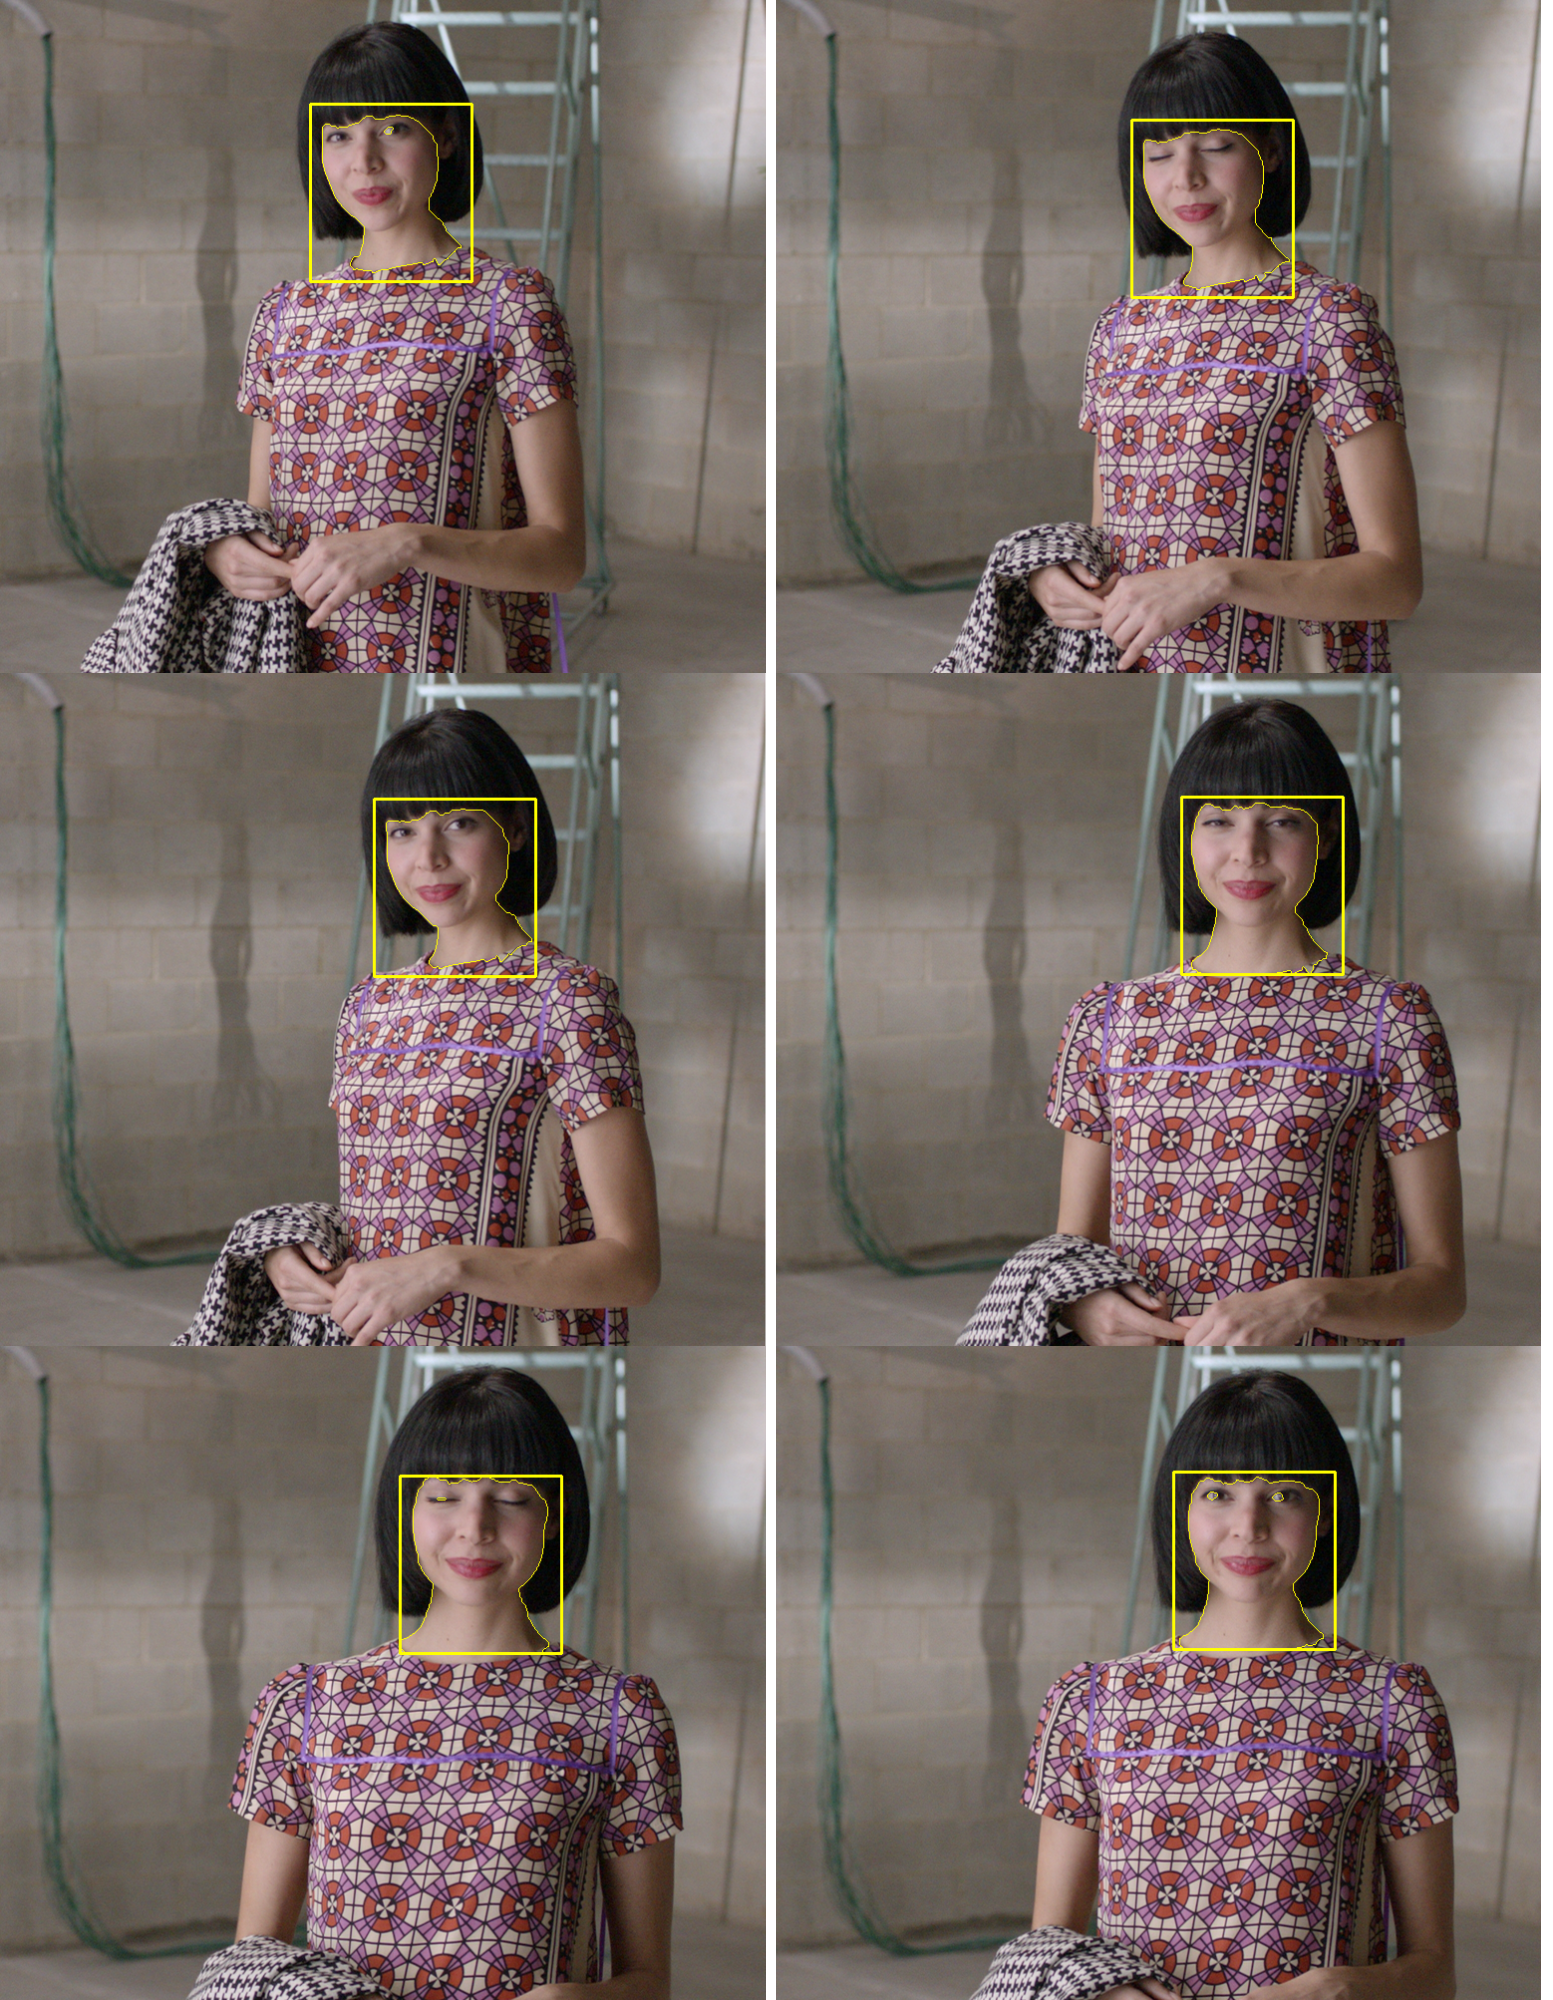
\includegraphics[width=1.00\textwidth]{../images/other_segm2.png}
      \label{othersegm1}
   \end{figure}

% ===================================================

\bibliographystyle{plain}
%\bibliography{tex/refs}
\begin{thebibliography}{99}

\bibitem{c12}
A. Shekhovtsov, I. Kovtun and V. Hlavac. Efficient MRF deformation model for non-rigid image matching, {\it Computer Vision and Pattern Recognition}. 2007.

\bibitem{c24}
B. Babenko, M.H. Yang, and S. Belongie. Visual Tracking with Online Multiple Instance Learning. {\it Computer Vision and Pattern Recognition}. 2009.

\bibitem{c5}
B. Horn and B. Schunck, Determining Optical Flow, {\it Artificial Intelligence}, 1981.

\bibitem{c22}
Brox, A. Bruhn, N. Papenberg, J. Weickert. High accuracy optical flow estimation based on a theory for warping. {\it European Conference in Computer Vision}. 2004.

\bibitem{c14}
C. Rother, V. Kolmogorov and A. Blake. Grabcut: Interactive foreground extraction using iterated graph cuts, {\it SIGGRAPH}. 2004.

\bibitem{c3}
E. Boros; P. Hammer and G. Tavares, Preprocessing of unconstrained quadratic binary optimization, {\it RUTCOR}, 2010.

\bibitem{c4}
E. Boros and P. Hammer, Pseudo-boolean optimization, {\it Discrete applied Mathematics.}, 2002.

\bibitem{c10}
F. Perbet and A. Maki, Homogeneus superpixels from random walks, {\it MVA.}, 2011.

\bibitem{c25}
J. Shi and C. Tomasi. Good features to track. {\it Conference on Computer Vision and Pattern Recognition }, 1994. 

\bibitem{c13}
J. Sun, N.N Shen and H.Y. Shum. Stereo matching using propagation belief, {\it TPAMI}. 2003.

\bibitem{c21}
M. Tao, J. Bai, P. Kohli, and S. Paris. SimpleFlow: A Non-iterative, Sublinear Optical Flow Algorithm, {\it Computer Graphics Forum, Eurographics}. 2012.

\bibitem{c9}
R. Achanta; A. Shaji; K. Smith; Aurelien Lucchi; P. Fua and S. Susstrunk, SLIC Superpixels compared to state of the art superpixel methods, {\it Discrete applied Mathematics.}, 2002.

\bibitem{c17}
S. Baker, D. Scharstein, J.P. Lewis, S. Roth, M.J. Black and R. Szeliski. A Database and Evaluation Methodology for Optical Flow, {\it International Journal Computer Vision}. 2013.

\bibitem{c23}
S. Hare, A. Saffari, and P.H.S. Torr, Struck: Structured Output Tracking with Kernels.  {\it International Conference on Computer Vision}. 2011.

\bibitem{c20}
T. Crivelli, P.-H. Conze, P. Robert, M. Fradet and P. Perez. Multi-step flow fusion: towards accurate and dense correpondence in long video shots, {\it British Conference Machine Vision}. 2012.

\bibitem{c7}
V. Lempitsky, S. Roth and C. Rother, Fusion Flow: Discrete-Continuos optimization for optical flow estimation, {\it Computer Vision and Pattern Recognition}, 2008.

\bibitem{c19}
W. Li, D. Cosker and M. Brown. An anchor patch based optimization framework for reducing optical flow drift in long image sequences, {\it Asian Conference on Computer Vision}. 2012.

\bibitem{c18}
Y. Boykov, M-P. Jolly. Interactive Graph Cuts for Optimal Boundary \& Region Segmentation of Objects in N-D images, {\it International Conference on Computer Vision}. 2013.

\bibitem{c16}
Y. Wu, J. Lim and M.-H. Yang. Online object tracking: A benchmark, {\it Computer Vision and Pattern Recognition}. 2013.

\end{thebibliography}

%adds the bibliography to the table of contents
\addcontentsline{toc}{chapter}
         {\protect\numberline{Bibliography\hspace{-96pt}}}

\end{document}
